% chktex-file 15
% chktex-file 17
\documentclass[lang=cn,10pt,color=blue]{elegantbook}

% === 风格约定 ===
% 表格/图片: 一律用 [ht]，不要用 [H]（避免页面空白）
% 金融变量: 用 \mathrm{}（如 \mathrm{ROE}, \mathrm{NPV}）
% 协方差/相关系数: 用 \operatorname{}（如 \operatorname{Cov}）
% 高亮标题: \textbf{\color{UnivColor} 【标题】}
% 数字: math mode 内空格不影响输出，可忽略
% ===============

\title{公司金融学笔记}
\subtitle{实物期权、证券估值与现代资产组合理论}

\author{Harry}
\institute{University}
\date{2026年5月}
\version{1.0}
\bioinfo{学科}{公司金融学 (Corporate Finance)}

\extrainfo{Myers (1977) 提出：项目真实价值 = 传统 NPV + 实物期权价值。}

\setcounter{tocdepth}{2}

\logo{logo-blue.png}
\cover{cover.jpg}

\usepackage{array}
\usepackage{booktabs} % beautiful tables
\usepackage{tabularx} % auto-wrapping tables
\newcolumntype{Y}{>{\raggedright\arraybackslash}X}

\definecolor{UnivColor}{RGB}{212,69,0}

\begin{document}

\maketitle
\frontmatter

\tableofcontents

\mainmatter

\chapter{实物期权 (Real Options)}

Myers (1977) 提出：项目真实价值 = 传统 NPV + 实物期权价值。在投资面临不确定性的情 景下，企业管理层拥有根据市场变化调整决策的期权，这种选择权能够为项目带来额外的价值。 

\section{实物期权的概念与分类}

在项目投资中，实物期权是指在未来面临不确定性时，公司所拥有的调整经营和投资决策 的权利。常用的分析方法为决策树分析法。 

\begin{table}[ht]
  \centering
  \caption{表 1: 实物期权的主要类型与特征}
  \renewcommand{\arraystretch}{1.4}
\begin{tabularx}{\textwidth}{lYY}
  \toprule
  类型 & 触发条件 & 典型应用场景 \\
  \midrule
  1. 拓展期权 (Expansion Option) & 市场需求增加 (Sales $\uparrow$),利润优于预期 & 开设新店、实施兼并与收购等 \\
  2. 放弃期权 (Abandonment Option) & 市场需求下滑 (Sales $\downarrow$),经营业绩欠佳 & 关停亏损业务、缩减生产产能等 \\
  3. 等待期权 (Timing Option) & 市场前景不确定,等待最优投资时点 & 延迟项目投资启动时点 \\
  \bottomrule
\end{tabularx}
\end{table}

\section{放弃期权例题分析}

\subsection{案例背景与基本参数}

预期某新项目未来10年，每年售出6,000单位产品，每单位带来50美元的净现金流。项目 的必要报酬率（折现率 $r_s$）为16\%，初始投资为 120万美元。 

\begin{itemize}
  \item Step 1：基本情景下的 NPV：不考虑任何调整弹性时的项目净现值为多少？

  \item Step 2：放弃期权边界分析：若第 1 年末可以以 100 万美元的价格变卖清算资产，在什么 销量水平下选择放弃是合理的？

  \item Step 3：含放弃期权的项目价值评估：若项目成功与失败概率各占 50\%，求包含放弃期权 时的项目 NPV 及其期权价值。
\end{itemize}

注. 核心边界条件：无论市场最终走向如何，第 1 年的销售量均能稳定达到 6,000 单位（即 t = 1 时的现 金流 CF 是确定的，不确定性仅从 t = 2 开始显现）。 

\subsection{基本情景下的 NPV 计算}

在基准情景（Base Case）下，项目不具备任何调整弹性，净现值计算如下： 

\textbf{\color{UnivColor} 【确定性基准 NPV】} 

$$
\mathrm{NPV} = - 120 + 30 \times \left[ \frac {1 - (1 + 16\%) ^ {- 10}}{16\%} \right] = - 120 + 30 \times 4.833 = 25 \text{万美元}
$$

\subsection{放弃期权的临界销售量确定}

在第1年末，决策者需要对比“继续经营9年的未来净现金流现值（P V）”与“立刻变卖资产 获得100 万美元的清算收益”： 

$$
50Q\times \left[\frac{1 - (1 + 16\%)^{-9}}{16\%}\right] <   1,000,000
$$

$$
5 0 Q \times 4. 6 0 7 <   1, 0 0 0, 0 0 0
$$

$$
Q <   \boxed {\frac {1 , 0 0 0 , 0 0 0}{5 0 \times 4 . 6 0 7} = 4, 3 4 1. 6 5 \text {单位}}
$$

求解临界销量 Q，得出\textbf{\color{UnivColor} 【放弃期权决策边界】}。 

结论：当市场低迷导致年销量低于 4, 341.65 单位时，立刻变卖资产相比继续经营更符合股东利 益。 

\subsection{含放弃期权的项目价值与期权价值}

若项目面临失败情景（年销售量下滑至 4,000 单位），由于 4, 000 < 4, 342 单位，公司应当 选择在第 1年末执行变卖放弃决策。 

\subsubsection{现金流决策树分支}

在 t = 0 时点初始投入 120 万美元。在 t = 1 时点确定收 30 万美元，然后进行决策： 

\begin{itemize}
  \item 成功分支（概率 50\%）：继续经营，在 $t = 2 \sim 10$ 年间每年获得现金流 30 万美元。

  \item 失败分支（概率 50\%）：变卖资产放弃，在 t = 1 年末清算回收 100 万美元。
\end{itemize}

\subsubsection{各期现金流折现（折回t = 0 时点）}

\begin{itemize}
  \item 第 1 年确定现金流折现：
\end{itemize}

$$
\mathrm{PV} _ {t = 1} = \frac {3 0}{1 . 1 6} = 2 5. 8 6 \text {万美元}
$$

\begin{itemize}
  \item 成功分支（持续经营9 年）折现：
\end{itemize}

$$
\mathrm{PV} _ {\text {成功}} = \frac {50 \% \times 3 0 \times 4 . 6 0 7}{1 . 1 6} = 5 9. 5 7 \text {万美元}
$$

\begin{itemize}
  \item 失败分支（第 1年末清算）折现：
\end{itemize}

$$
\mathrm{PV} _ {\text { 失败 }} = \frac {50 \% \times 100}{1.16} = 43.10 \text { 万美元 }
$$

\subsubsection{衡量期权与期权独立价值测算}

对照组：无期权净现值（失败时继续经营9 年，每年带来 20万美元现金流）为： 

$$
\mathrm{NPV} _ {\text {无期权}} = - 120 + 25.86 + 59.57 + \frac {50 \% \times \frac {4,000 \times 50}{10,000} \times 4.607}{1.16} = 5.14 \text {万美元}
$$

引入放弃期权决策后，项目价值计算如下： 

\subsubsection{【含期权NPV 与期权净价值】}

$$
\mathrm{NPV} _ {\text {含期权}} = - 1 2 0 + 2 5. 8 6 + 5 9. 5 7 + 4 3. 1 0 = 8. 5 3 \text {万美元}
$$

$$
\text { 期权价值 } = \mathrm{NPV} _ {\text { 含期权 }} - \mathrm{NPV} _ {\text { 无期权 }} = 8. 5 3 - 5. 1 4 = 3. 3 9 \text {   万美元   }
$$

\section{例题计算结果归纳}

\begin{table}[ht]
  \centering
  \caption{表 2: 各种决策场景下的项目净现值对比}
  \renewcommand{\arraystretch}{1.4}
\begin{tabularx}{\textwidth}{lYY}
  \toprule
  评估指标 & 数值大小 & 决策状态与学术含义 \\
  \midrule
  基准 NPV(无不确定性,销售量确定为 6,000) & +25.00 万美元 & 确定性情景下的项目理论价值 \\
  无期权 NPV(50/50 概率,面临失败时必须继续经营) & +5.14 万美元 & 传统 NPV 决策,低估了项目在恶劣环境下的价值 \\
  含放弃期权 NPV(50/50 概率,失败时选择清算) & +8.53 万美元 & 引入管理决策弹性后的项目真实商业价值 \\
  放弃期权的独立价值 & +3.39 万美元 & 放弃权本身带来的非对称风险对冲价值 \\
  \bottomrule
\end{tabularx}
\end{table}

注. 历年真题考点深度归纳、三类期权（拓展、放弃、等待）的通用解题套路、以及决策树标准画法规范 将在后续进行扩展。 

\chapter{债券估值 (Bond Valuation)}

注. 大纲导读：证券估值 债券估值——核心要点包括：债券基本定义、债券契约条款、债券分类、标准 定价公式、三种收益率（票面收益率、当前收益率、到期收益率Y TM）、可转换债券估值理论以及历年 真题精解。 

本章详细内容尚未正式录入。目前相关复习图表素材已就位（图50至图65，共16张），待 后续正式整理债券估值章节内容时，将统一按照规范的学术排版格式进行扩展与深度整理。 

\chapter{股票估值 (Stock Valuation)}

股票估值是公司金融学和资产定价的核心内容。本章梳理了绝对估值模型（股利贴现模型 DDM、成长机会净现值模型NPVGO）与相对估值模型（市盈率PE、企业价值倍数EV/EBITDA） 的核心理论，结合杜邦传导链深度剖析了再投资决策对企业股东价值创造的影响，并配以各大 名校的历年真题进行实战演练。 

\section{股票估值模型选择导引}

在进行股票估值时，应当首先根据现金流特征识别现金流形态，然后再选择合适的估值模 型，避免盲套公式。 

\section{股票基础知识}

\subsection{股票所有权特征}

\begin{itemize}
  \item 本质属性：股票代表投资者对公司的股权投资，享有公司的净资产剩余索取权。
\end{itemize}

\begin{table}[ht]
  \centering
  \caption{表 3: 股票估值模型选用矩阵}
  \renewcommand{\arraystretch}{1.4}
\begin{tabularx}{\textwidth}{llYY}
  \toprule
  题目特征/现金流形态 & 优先选用模型 & 核心计算公式 & 核心操作要点与常见陷阱 \\
  \midrule
  股利固定不变 & 固定股利模型(永续年金) & $P_0 = \dfrac{D_1}{r_s}$ & 确认属于永续固定红利,直接按永续年金进行折现定价。 \\
  股利固定增长 & 戈登增长模型(Gordon) & $P_0 = \dfrac{D_1}{r_s - g}$ & 务必分清提供的是历史股利 $D_0$ 还是下一期预期股利 $D_1$ 。若为 $D_0$,需乘以 $(1 + g)$ 。 \\
  增长率分阶段变动 & 两阶段增长模型 (DDM) & $P_0 = \sum_{t=1}^{n} \dfrac{D_t}{(1 + r_s)^t} + \dfrac{P_n}{(1 + r_s)^n}$ & 绘制现金流时间轴:对高增长期股利逐个折现,对永续期股利利用戈登公式计算终值 $P_n$ 并折现。 \\
  强调盈利、再投资率及 ROE & 成长机会净现值模型(NPVGO) & $V_0 = \dfrac{E_1}{r_s} + NPVGO$ & 比较新增资产回报率 ROE 与必要报酬率 $r_s$:只有 $ROE > r_s$ 时,留存再投资才会创造价值。 \\
  给出同行业 PE /EPS 等数据 & 相对估值模型(PE) & $PE = \dfrac{P}{EPS}$ & 厘清分母盈利口径是静态历史 $E_0$、预期动态 $E_1$ 还是滚动近四季 TTM。 \\
  \bottomrule
\end{tabularx}
\end{table}

\subsection{基本股东权益：}

\begin{itemize}
  \item 剩余索取权：公司清算时，普通股股东在清偿债务和优先股之后，对剩余资产拥有分 配权。

  \item 剩余控制权：股东通过股东大会对公司的重大经营方针、董事选举等进行投票决策。

  \item 优先认股权：当公司发行新股时，现有股东享有按比例优先认购的权利，以防止股权 被稀释。
\end{itemize}

\subsection{普通股投票权机制与制度对比}

在董事会选举中，不同的投票权设计会深刻影响大股东与中小股东利益的博弈。 

\subsubsection{简单多数投票制（Straight Voting）}

每股对每一位董事候选人均拥有 1 票投票权，各席位分别选举。要确保选出 1 名董事，大 股东所持有的最少股数比例必须满足： 

$$
\boxed {x > 50 \%} \quad (\text{即占总股数的} \frac {1}{2} + 1 \text{股})
$$

注. 简单多数投票制下，大股东能够实现完全控制。要确保选出1名董事，其持股比例必须拥有绝对多数 优势。 

\subsubsection{累计投票制（Cumulative Voting）}

若公司拟选举 N 名董事，则股东持有的每 1 股股份均拥有 N 票投票权，股东可以将全部票 数集中投给一人或分投多人。此项机制极大地保护了中小股东的话语权。要确保选出 1 名董事， 所需要的最少持股比例x 如下： 

$$
\boxed {x > \frac {1}{N + 1}}
$$

学术推导：设某股东持股比例为x，拟通过将所有票数集中投给1位候选人以确保其当选。该候 选人得票数为x N。为了确保其能够击败其他竞争对手，其得票必须超过对手在剩余席位上所 能平均分配的最大票数： 

【累计投票制持股临界比例推导】 

$$
x \cdot N > \frac {(1 - x) \cdot N}{N} = 1 - x
$$

$$
x N + x > 1
$$

$$
x > \boxed {\frac {1}{N + 1}}
$$

\subsection{优先股的特征与局限}

\begin{itemize}
  \item 非对称性：在剩余资产索取和股利分配顺序上优先于普通股；但在公司治理上通常没有表 决权（无剩余控制权）。
\end{itemize}

\section{绝对估值模型：股利贴现模型（DDM）}

\subsection{股利贴现模型的基本原理}

股票的内在价值（V0）等于未来所有预期派发股利的现值之和： 

$$
\boxed {V _ {0} = \sum_ {t = 1} ^ {\infty} \frac {D _ {t}}{(1 + r _ {s}) ^ {t}}} = \frac {D _ {1}}{1 + r _ {s}} + \frac {D _ {2}}{(1 + r _ {s}) ^ {2}} + \dots
$$

【DDM横截性收敛条件（无资产泡沫前提）】 

$$
\lim _ {n \to \infty} \frac {V _ {n}}{(1 + r _ {s}) ^ {n}} = 0
$$

在任意相邻的时点间，股票价值均满足如下的递推关系： 

$$
V _ {t} = \frac {D _ {t + 1} + V _ {t + 1}}{1 + r _ {s}}
$$

\subsection{股利贴现模型的三种子模型}

根据公司生命周期的不同阶段，DDM 细分为三种常见的现金流结构模型。 

\begin{table}[ht]
  \centering
  \caption{表 4: DDM三种子模型特征与定价公式}
  \renewcommand{\arraystretch}{1.4}
\begin{tabularx}{\textwidth}{llYY}
  \toprule
  发展阶段 & 模型名称 & 核心特征描述 & 标准定价公式 \\
  \midrule
  成熟稳健期 & 固定股利模型 & 预期未来各期股利保持恒定(相当于永续年金) & $P_0 = \dfrac{D_1}{r_s}$ \\
  高速成长永续期 & 固定增长模型(戈登增长模型) & 股利以恒定的增长率 $g$ 永续增长(必须满足必要报酬率$r_s > g$) & $P_0 = \dfrac{D_1}{r_s - g}$ \\
  初创与转型期 & 两阶段增长模型 & 增长率分段变化,前高后低。初期不规则高增长,后期转入永续平稳增长阶段。 & $\begin{aligned}
P_0 &= \sum_{t=1}^{n} \frac{D_t}{(1+r_s)^t} + \frac{V_n}{(1+r_s)^n} \\[2pt]
\text{其中 } D_1 &= D_0(1+g),\quad V_n = \frac{D_{n+1}}{r_s - g_2}
\end{aligned}$ \\
  \bottomrule
\end{tabularx}
\end{table}

\subsection{戈登增长模型（Gordon Growth Model）学术推导与参数测算}

\subsubsection{【戈登增长模型学术推导（等比级数收敛法）】}

设公司未来各期预期分红以固定增长率 g 增长，即 $D _ { t } = D _ { 1 } ( 1 + g ) ^ { t - 1 }$ 。若投资者要求的股 权必要报酬率为 $r _ { s }$ （且满足收敛条件 $r_s > g$），将各期红利代入绝对估值DDM 模型： 

$$
\begin{aligned}
  V _ {0} &= \frac {D _ {1}}{1 + r _ {s}} + \frac {D _ {1} (1 + g)}{(1 + r _ {s}) ^ {2}} + \frac {D _ {1} (1 + g) ^ {2}}{(1 + r _ {s}) ^ {3}} + \dots + \frac {D _ {1} (1 + g) ^ {t - 1}}{(1 + r _ {s}) ^ {t}} + \dots \\[1.2ex]
  &= \sum_ {t = 1} ^ {\infty} \frac {D _ {1} (1 + g) ^ {t - 1}}{(1 + r _ {s}) ^ {t}} \\[1.2ex]
  &= \frac {D _ {1}}{1 + r _ {s}} \sum_ {t = 1} ^ {\infty} \left(\frac {1 + g}{1 + r _ {s}}\right) ^ {t - 1}
\end{aligned}
$$

由于必要报酬率大于增长率 $r_s > g$，则公比 $q = \frac{1 + g}{1 + r_s} < 1$。根据无限项等比级数收敛公式 $\textstyle \sum _ { n = 0 } ^ { \infty } q ^ { n } = { \frac { 1 } { 1 - q } }$ ，该级数收敛于： 

$$
\sum_ {t = 1} ^ {\infty} \left(\frac {1 + g}{1 + r _ {s}}\right) ^ {t - 1} = \frac {1}{1 - \frac {1 + g}{1 + r _ {s}}} = \frac {1 + r _ {s}}{r _ {s} - g}
$$

代入原式即可化简得出经典的戈登永续增长定价公式： 

$$
\boxed {V _ {0} = \frac {D _ {1}}{r _ {s} - g}} \quad \text {(或写为: } \boxed {V _ {0} = \frac {D _ {0} (1 + g)}{r _ {s} - g}} \text {)}
$$

在实际应用中，如何科学地确定未来的分红 $D _ { 1 }$ 、必要报酬率 $r _ { s }$ 以及增长率 $g$ 是核心技术 点。 

1. 下期红利 $D _ { 1 }$ 与留存比率 b 

利用预期每股收益 $\mathrm { E P S _ { 1 } }$ 以及再投资留存比例b，可将股利表示为： 

$$
D _ {1} = \mathrm{EPS} _ {1} \times (1 - b)
$$

其中，留存比率 b = 1 - 股利支付率。 

2. 内在永续增长率 g 与必要报酬率 $r _ { s }$ 

公司能够保持增长的原因，在于管理层将部分利润留存并再次投入高回报项目中： 

\textbf{\color{UnivColor} 【戈登模型成长增长率与必要报酬率分解】} 

$$
\boxed {g = \mathrm {R O E} \times b}
$$

$$
\boxed {r _ {s} = \frac {D _ {1}}{P _ {0}} + g}
$$

\section{两阶段股利贴现模型案例分析}

\subsection{案例背景与参数}

DG公司今年刚刚发放了每股 $D _ { 0 } = 1 . 0 0$ 美元的红利。预计未来3年（高成长阶段）红利每 年高速增长 $g _ { 1 } = 2 5 \%$ 。从第 4 年开始，红利增长率降至稳定永续阶段 $g _ { 2 } = 5 \%$ 。投资者要求的 必要报酬率 $r _ { s } = 2 0 \%$ 。 

\subsection{现金流时点建模}

两阶段估值现金流时间轴及定价逻辑如下： 

\begin{itemize}
  \item $t = 0 \colon D _ { 0 } = 1 . 0 0$ 美元
\end{itemize}

$\bullet \ t = 1 : D _ { 1 } = D _ { 0 } ( 1 + g _ { 1 } ) = 1 . 2 5$ 美元，折现至 t = 0 为 $\frac{1.25}{1.20}$

$\bullet \ t = 2 \colon D _ { 2 } = D _ { 1 } ( 1 + g _ { 1 } ) = 1 . 5 6 2 5$ 美元，折现至 t = 0 为 $\textstyle { \frac { 1 . 5 6 2 5 } { 1 . 2 ^ { 2 } } }$ 

$\bullet \ t = 3 : D _ { 3 } = D _ { 2 } ( 1 + g _ { 1 } ) = 1 . 9 5 3$ 美元，折现至 t = 0 为 $\frac { 1 . 9 5 3 } { 1 . 2 ^ { 3 } }$ 

\begin{itemize}
  \item $t = 4 \div$ 进入永续增长阶段，首期股利 $D _ { 4 } = D _ { 3 } ( 1 + g _ { 2 } ) = 2 . 0 5 1$ 美元。
\end{itemize}

在第 3 年末，永续期现金流的现值为 $\displaystyle V _ { 3 } = \frac { D _ { 4 } } { r _ { s } - g _ { 2 } }$ ，其折回 t = 0 时点为 $\frac { V _ { 3 } } { 1 . 2 ^ { 3 } }$ 

\subsection{股票价值与指标测算}

\subsubsection{股票价值计算}

首先计算高增长期各年的具体红利金额： 

\begin{itemize}
  \item $D _ { 1 } = 1 . 2 5$ 美元， $D _ { 2 } = 1 . 5 6 2 5$ 美元， $D _ { 3 } = 1 . 9 5 3$ 美元。
\end{itemize}

$\bullet D _ { 4 } = D _ { 3 } \times ( 1 + g _ { 2 } ) = 2 . 0 5 1$ 美元。 

利用上述参数计算两阶段 DDM 内在价值： 

\textbf{\color{UnivColor} 【两阶段DDM 内在价值定价】} 

$$
V _ {3} = \frac {D _ {4}}{r _ {s} - g _ {2}} = \frac {2 . 0 5 1}{20 \% - 5 \%} = 1 3. 6 7 \text{美元}
$$

$$
V _ {0} = \frac {1 . 2 5}{1 . 2 0} + \frac {1 . 5 6 2 5}{1 . 2 0 ^ {2}} + \frac {1 . 9 5 3}{1 . 2 0 ^ {3}} + \frac {1 3 . 6 7}{1 . 2 0 ^ {3}} = 1. 0 4 + 1. 0 9 + 1. 1 3 + 7. 9 1 = 1 1. 1 7 \text {美元}
$$

2. 当期股利收益率 

$$
\text{股利收益率} = \frac {D _ {1}}{P _ {0}} = \frac {1 . 2 5}{1 1 . 1 7} \approx 1 1. 1 9 \%
$$

3. 投资者持有一年后的预期股票价格 $V _ { 1 }$ 与资本利得率 

\begin{itemize}
  \item 方法一：依据 DDM价值增值递推关系
\end{itemize}

$$
V _ {1} = V _ {0} \times (1 + r _ {s}) - D _ {1} = 1 1. 1 7 \times 1. 2 0 - 1. 2 5 = 1 2. 1 5 \text { 美元 }
$$

\begin{itemize}
  \item 方法二：依据报酬率分解公式反推
\end{itemize}

$$
\text{资本利得率} = r _ {s} - \text{股利收益率} = 20 \% - 11.19 \% = 8.81 \%
$$

$$
V _ {1} = V _ {0} \times (1 + 8. 8 1 \%) = 1 1. 1 7 \times 1. 0 8 8 1 \approx 1 2. 1 5 \text { 美元 }
$$

注. 易错点：投资者经常误认为资本利得率在任何时候都等于股利增长率。请注意：在两阶段模型中，当 前处于高速增长的第一阶段，并非单阶段永续模型。因此，第一年的资本利得率（8.81\%）既不等于高增 长率 $g _ { 1 } = 2 5 \%$ ，也不等于永续期增长率 $g _ { 2 } = 5 \%$ 。 

\section{成长机会净现值（NPVGO）模型}

\subsection{NPVGO 模型的基本公式}

该模型将公司的整体价值解构为两部分： 

【成长机会净现值(NPVGO)分解模型】 

$$
\boxed {V _ {0} = \underbrace {\frac {E _ {1}}{r _ {s}}} _ {\text {现金牛价值}} + \mathrm {N P V G O}}
$$

$\frac { E _ { 1 } } { r _ { s } }$ （零增长基准价值）：将公司视为“现金牛”（Cash Cow）时的资产清算派息价值。即假设 公司不做任何留存再投资（b = 0），将所有盈余作为股利发放。 

\begin{itemize}
  \item NPVGO（成长机会净现值）：衡量企业实施留存收益再投资决策后，相比零增长基准线所 创造（或摧毁）的股东价值。
\end{itemize}

\subsection{留存决策与股东价值创造的辨析}

注. 结论：增加留存比例会使未来盈利增速加快，但并不制造股价上涨。留存再投资能否创造价值，取决 于新增投资的回报率。 

\begin{table}[ht]
  \centering
  \caption{表 5: ROE 与必要报酬率关系的影响}
  \renewcommand{\arraystretch}{1.4}
\begin{tabularx}{\textwidth}{llYY}
  \toprule
  ROE与$r_s$关系 & NPVGO正负号 & 最终股价变动效应 & 学术结论与管理启示 \\
  \midrule
  $ROE > r_s$ & NPVGO>0 & 股价上涨 & 创造价值。留存资金能够赚取超额回报,应提高留存比率b。 \\
  $ROE = r_s$ & NPVGO=0 & 股价不变 & 价值中性。项目回报仅能弥补股东机会成本,留存与否无差异。 \\
  $ROE < r_s$ & NPVGO<0 & 股价下跌 & 摧毁价值。再投资收益率过低,应当进行100\%分红。 \\
  \bottomrule
\end{tabularx}
\end{table}

\subsection{g = ROE  b 的杜邦传导链学术推导}

\begin{itemize}
  \item 假设前提：新增再投资资本的盈利能力与公司现有资产相同（即边际 ROE 等于平均 ROE）。

  \item 传导步骤：
\end{itemize}

1. 留存利润增加股东权益： $\Delta S = \mathrm { N I _ { 0 } } \times b$。 

2. 维持负债结构，总资产同比例扩张： $\Delta A = \Delta S \times \mathrm{EM}_{0}$ 。 

3. 新增资产按周转效率创造销售额： $\Delta \mathrm { S a l e s } = \Delta A \times \mathrm{ATO}$。 

4. 新增收入按净利润率转化为净利润： $\Delta \mathrm { N I } _ { 1 } = \Delta \mathrm { S } \mathrm { a l e s } \times \mathrm { P M }$。 

5. 两侧相乘化简，利用杜邦分解式 $\mathrm { E M } \times \mathrm { A T O } \times \mathrm { P M } = \mathrm { R O E }$ 可得： 

$$
g = \frac {\Delta \mathrm {N I} _ {1}}{\mathrm {N I} _ {0}} = \mathrm {R O E} \times b
$$

\subsection{持续性与有限期两类 NPVGO 计算场景}

\begin{table}[ht]
  \centering
  \caption{表 6: 两类 NPVGO计算方法对比}
  \renewcommand{\arraystretch}{1.4}
\begin{tabularx}{\textwidth}{lYY}
  \toprule
  分类形态 & 适用商业场景 & 核心计算步骤与路径 \\
  \midrule
  永续持续性增长 & 公司以固定的留存比率$b$持续进行项目再投资。 & 1. 直接套用戈登增长模型计算当期股价:$P_0 = \dfrac{E_1(1-b)}{r_s - ROE \cdot b}$\newline 2. 根据定义反推:NPVGO=$P_0 - \dfrac{E_1}{r_s}$ \\
  有限期独立项目 & 公司在某一时点投入一笔资金,项目存续若干年后结束。 & 1. 计算该独立投资项目在投资时点的净现值:NPV项目\newline 2. 将项目现值折回至当期$t = 0$:NPVGO=$\dfrac{\text{NPV}_{\text{项目}}}{(1 + r_s)^t}$\newline 3. 加总求值:$P_0 = \dfrac{E_1}{r_s} + \text{NPVGO}$ \\
  \bottomrule
\end{tabularx}
\end{table}

\section{Lane Supermarkets 案例分析（持续性 NPVGO）}

\subsection{案例背景}

Lane Supermarkets 共有发行在外的普通股 10,000 股。公司当前每年净利润恒定为 100,000 美元，股权必要报酬率 $r _ { s } = 1 6 \%$ 。现拟对比两套财务策略： 

\begin{itemize}
  \item 方案一（零增长/现金牛）：不做任何留存再投资，100\%净利润均作为股利发放。

  \item 方案二（持续拓展）：每年留存净利润的 $b = 2 0 \%$ ，用于投资 $\mathrm { R O E } = 1 0 \%$ 的新项目。
\end{itemize}

\subsection{定价与 NPVGO 测算}

\subsubsection{方案一（现金牛）下的基准股价}

\subsubsection{【零增长方案下股价】}

$$
P _ {0} ^ {\text {方案一}} = \frac {E _ {1}}{r _ {s}} = \frac {1 0 0 , 0 0 0 / 1 0 , 0 0 0}{16 \%} = 6 2. 5 0 \text {美元}
$$

\subsubsection{方案二（拓展方案）下的价值损毁测算}

由于 $\mathrm { R O E } ( 1 0 \% ) < r _ { s } ( 1 6 \% )$ ，留存资金再投资将使得股东价值受损： 

\subsubsection{【拓展方案下的价值损毁测算】}

$$
P _ {0} ^ {\text {方案二}} = \frac {D _ {1}}{r _ {s} - g} = \frac {E _ {1} \times (1 - b)}{r _ {s} - \mathrm{ROE} \times b} = \frac {10 \times 80 \%}{16 \% - 2 \%} \approx 57.14 \text {美元}
$$

$$
\mathrm{NPVGO} = P _ {0} ^ {\text {方案二}} - \frac {E _ {1}}{r _ {s}} = 5 7. 1 4 - 6 2. 5 0 = - 5. 3 6 \text {美元}
$$

\section{Stambaugh 公司案例分析（有限期 NPVGO）}

\subsection{案例背景}

Stambaugh 公司当前每股收益 $E _ { 0 } = 8 . 2 5$ 美元，占分红100\%。现有一项新投资机会：在 $t = 1$ 时点留存每股 1.60 美元作为项目初始投资，该项目存续 2 年，能使 t = 2,3 时的每股收益分别 比原基准上升 2.10美元和 2.45美元，之后盈利恢复原基准水平。投资者要求回报率 $r _ { s } = 1 2 \%$ 。 

\subsection{股票价值递增分析}

\subsubsection{不进行投资时的每股价值（零增长现金牛基准）}

$$
V _ {0} = \frac {E _ {1}}{r _ {s}} = \frac {8 . 2 5}{12 \%} = 6 8. 7 5 \text{美元}
$$

\subsubsection{进行投资后股票的每股价值}

在第 1年末 t = 1 时，项目的净现值为 $\mathrm { N P V _ { 1 } }$ 。将其折回当期得到NPVGO溢价并定价： 

\textbf{\color{UnivColor} 【一次性项目 NPV与NPVGO估值】} 

$$
\mathrm{NPV} _ {1} = - 1. 6 0 + \frac {2 . 1 0}{1 + 12 \%} + \frac {2 . 4 5}{(1 + 12 \%) ^ {2}} = 2. 2 3 \text{美元}
$$

$$
\mathrm{NPVGO} = \frac {\mathrm{NPV} _ {1}}{1 + r _ {s}} = \frac {2 . 2 2 8}{1 . 1 2} \approx 1. 9 9 \text { 美元 }
$$

$$
V _ {0} = \frac {E _ {1}}{r _ {s}} + \mathrm{NPVGO} = 6 8. 7 5 + 1. 9 9 = 7 0. 7 4 \text {美元}
$$

\section{相对估值模型：市盈率（PE）估值法}

\subsection{市盈率与理论估值推导}

市盈率（Price-to-Earnings Ratio, PE）是相对估值乘数法的核心指标： 

$$
\boxed {\mathrm {P E} = \frac {P}{\mathrm {E P S}}, \quad \text {其倒数为盈利收益率:} \frac {1}{\mathrm {P E}} = \frac {\mathrm {E P S}}{P}}
$$

由绝对定价公式 $\displaystyle { P _ { 0 } } = \frac { { E _ { 1 } } \left( 1 - b \right) } { { r _ { s } } - g }$ ，可以推导得出动态与静态市盈率理论值： 

【理论市盈率与基本面因子关联公式】 

$$
\text { 预期 / 动态市盈率: } \boxed {\frac {P _ {0}}{E _ {1}} = \frac {1 - b}{r _ {s} - g}}
$$

$$
\text { 历史/静态市盈率: } \boxed {\frac {P _ {0}}{E _ {0}} = \frac {(1 - b) (1 + g)}{r _ {s} - g}}
$$

\subsection{三种盈利计量口径与因素影响}

\begin{table}[ht]
  \centering
  \caption{表7: 三种市盈率盈利口径比对}
  \renewcommand{\arraystretch}{1.4}
\begin{tabularx}{\textwidth}{lYY}
  \toprule
  指标名称 & 分母盈利口径定义 & 优缺点分析 \\
  \midrule
  静态/历史市盈率(Trailing PE) & $E_0$:上一年度已披露的确定年度每股收益 & 数据百分百确定、无预测偏差;但反映的信息滞后。 \\
  动态/预期市盈率(Forward PE) & $E_1$:市场预估的下一期年度每股收益 & 反映对未来的增长预期;但严重依赖主观预测偏差。 \\
  滚动市盈率(TTM PE) & $E_{TTM}$:最近已披露的连续4个季度每股收益之和 & 能够实时反映最新滚动的盈利状态;但易受季节性波动干扰。 \\
  \bottomrule
\end{tabularx}
\end{table}

\subsection{会计存货计量政策的偏差效应}

在物价持续上涨（通货膨胀）宏观环境下，采用先进先出（FIFO）与后进先出（LIFO）核 算将对账面 PE产生非真实干扰。 

\begin{table}[ht]
  \centering
  \caption{表 8: 市盈率关键决定因子变动效应}
  \renewcommand{\arraystretch}{1.4}
\begin{tabularx}{\textwidth}{llYY}
  \toprule
  变动驱动因子 & 变动方向 & 对PE变动方向的影响 & 经济学底层逻辑解释 \\
  \midrule
  再投资成长机会(g) & $g \uparrow$ & $PE \uparrow$ & 未来盈利潜力大,分母$r_s - g$变小,投资者愿意支付更高估值溢价。 \\
  公司经营特有风险($r_s$) & $r_s \uparrow$ & $PE \downarrow$ & 股东要求的风险溢价提高,导致贴现率升高,股价下降。 \\
  宏观无风险利率($r_f$) & $r_f \uparrow$ & $PE \downarrow$ & 利率上涨通过无风险资产的替代效应推升整体折现率$r_s$。 \\
  会计保守政策 & 会计越保守 & $PE \uparrow$ & 保守政策会压低账面收益EPS,在市价不变下导致PE被动升高。 \\
  \bottomrule
\end{tabularx}
\end{table}

\begin{table}[ht]
  \centering
  \caption{表 9: 不同存货计价方法财务影响比对}
  \renewcommand{\arraystretch}{1.4}
\begin{tabularx}{\textwidth}{llYY}
  \toprule
  存货计价核算方法 & 销售成本 (COGS) 变动 & 账面净利润 (E) 表现 & 期末存货及总资产表现 \\
  \midrule
  先进先出 (FIFO) & 偏低(结转早期低价存货) & 高(盈利虚高) & 偏高(总资产估值更贴近市价) \\
  后进先出 (LIFO) & 偏高(结转近期通胀存货) & 低(报表较保守) & 偏低(资产账面价值滞后) \\
  \bottomrule
\end{tabularx}
\end{table}

\subsection{跨资本结构估值指标：EV/EBITDA}

\begin{table}[ht]
  \centering
  \caption{表 10: PE 与 EV/EBITDA 估值指标对比分析}
  \renewcommand{\arraystretch}{1.4}
\begin{tabularx}{\textwidth}{lYY}
  \toprule
  比较维度 & 市盈率估值倍数 (PE) & 企业价值倍数 (EV/EBITDA) \\
  \midrule
  分子口径 & 仅考虑股权价值(对债权人不适用)。 & 考虑企业整体价值(股权+债权)。 \\
  资本结构差异 & 极易受财务杠杆高低利息费用的干扰。 & 免受财务杠杆影响。分子含负债,分母在利息扣除前。 \\
  折旧政策差异 & 会受到折旧摊销年限与会计方法改变的影响。 & 免受折旧方法影响。分母将折旧与摊销项加回。 \\
  税收政策差异 & 受税率变动、税收优惠直接冲击。 & 弱化税率差异干扰。分母在所得税扣除之前,因此不直接受所得税费用影响。 \\
  \bottomrule
\end{tabularx}
\end{table}

\subsection{股利支付率变动对股价的非对称效应案例}

注. 案例背景：某公司股票当前 $\mathrm{EPS}_0 = 1.00$ 元，当前市价 $P_0 = 10.00$ 元。当期股利支付率 $d = 5 0 \%$ ，再 投资回报率 $\mathrm { R O E } = 1 0 \%$ 。必要报酬率 $r _ { s } = 1 0 . 2 5 \%$ 。若公司决定降低分红，将股利支付率下调至 30\%（即留存比率 $b'$ 提高为70\%）： 

\textbf{\color{UnivColor} 【提高留存比例（降息）后的价值重估】} 

$$
g ^ {\prime} = \mathrm{ROE} \times b ^ {\prime} = 10 \% \times 70 \% = 7 \%
$$

$$
D _ {1} ^ {\prime} = E _ {0} \left(1 + g ^ {\prime}\right) \times d ^ {\prime} = 1. 0 0 \times 1. 0 7 \times 30 \% = 0. 3 2 1 \text {元}
$$

$$
P _ {0} ^ {\prime} = \frac {D _ {1} ^ {\prime}}{r _ {s} - g ^ {\prime}} = \frac {0.321}{10.25\% - 7\%} = \frac {0.321}{3.25\%} \approx 9.88 \text{元}
$$

\begin{itemize}
  \item 学术机理解析：由于项目边际 $\mathrm { R O E } ( 1 0 \% ) < r _ { s }$ (10.25\%)，提高留存属于价值损毁决策，导 致股价从原先的 10.00 元下降至 9.88 元。
\end{itemize}

\section{历年考研真题与详解}

案例 1 (2025 清华：存货计价方法对报表的影响). 当价格水平持续上升时，与采用后进先出法 （LIFO）核算的公司相比，采用先进先出法（FIFO）核算的公司财务报表会呈现何种变化？（） 

A.总资产和净利润都低 

B.总资产和净利润都高 

C.总资产低，净利润高 

D.总资产高，净利润低

\textbf{\color{UnivColor} 【答案】} B

\textbf{\color{UnivColor} 【解析】}物价上涨时，FIFO 方法先结转早期相对低价采购的存货成本，导致销售成本 COGS 偏 低，从而使期末净利润账面显著偏高；同时，尚未售出并留在资产负债表上的存货多为后期高 价采购的产品，导致期末存货资产账面估值偏高。 

案例 2 (2020 人大：低市盈率特征成因辨析). 中国工商银行的股票市盈率一直处于较低水平， 在A 股市场上市公司中处于相对较低区间，以下针对低市盈率的解释中，最不可能成立的是（） A.公司会计政策过于激进 B.公司的增长机会极少 C.股东所要求的必要报酬率 $r _ { s }$ 较低 D. 银行不良贷款等经营风险偏高 

\textbf{\color{UnivColor} 【答案】} C 

\textbf{\color{UnivColor} 【解析】} 由理论公式分析可知，预期/动态市盈率满足 $\displaystyle \frac { P _ { 0 } } { E _ { 1 } } = \frac { 1 - b } { r _ { s } - g }$ ，如果必要报酬率 $r _ { s }$ 降低，会 使分母 $r _ { s } \mathrm { ~ - ~ } g$ 减小，在其他条件不变下，反而会推高股价与 PE 估值。故 C 最不可能成立。 

案例 3 (2020/2021 人大：所得税待遇对企业价值乘数的影响). （判断题）运用企业价值倍数 （EV/EBITDA）估计公司整体业务价值时，不同公司在所得税待遇方面存在的差异不会对该乘数 产生直接影响。（） 

\textbf{\color{UnivColor} 【答案】} 正确 

\textbf{\color{UnivColor} 【解析】} 企业价值倍数分母中的 EBITDA 代表的是息税折旧及摊销前利润，此时尚未扣除企业 的所得税开支，因此能够直接剔除不同公司间所得税率及税负待遇差异的干扰。 

案例 4 (2021  中财：名词解释——市净率 PB). 试解释市净率 (Price-to-Book Ratio, PB) 的金融含 义与数理联系。 

\textbf{\color{UnivColor} 【答案】} 

$$
\mathrm{PB} = \frac {P}{\mathrm{BPS}} = \frac {\text { 每股市场价格 }}{\text { 每股账面净资产 }}
$$

1. 含义：市净率表示投资者愿意为公司每 1 元账面净资产支付的市场价格。 

2. 内在联系：根据内在公式可拆解为： $\mathrm { P B } = \mathrm { P E } \times \mathrm { R O E }$ 。这说明市净率的高低最终依旧取决 于资产能够创造盈余的效率（即ROE的水平）。 

案例 5 (2024  上财：理论市盈率与投资决策). 某公司股票当前价格是 20 元，最近一期 $\mathrm{EPS}_0 = 0.40$ 元，每股股利 $D _ { 0 } = 0 . 3 2$ 元。预计以后每股收益按每年 g = 5\% 增长，期望必要报酬率为 $r _ { s } = 1 0 \%$ 。求：（1）该公司股票的理论市盈率；（2）结合实际市盈率给出投资决策建议。 

\subsubsection{【答案/解析】}

1. 计算下一期预期红利： $D _ { 1 } = D _ { 0 } \times ( 1 + g ) = 0 . 3 2 \times 1 . 0 5 = 0 . 3 3 6$ 元。 

2. 计算合理理论估值： $\displaystyle V _ { 0 } = \frac { D _ { 1 } } { r _ { s } - g } = \frac { 0 . 3 3 6 } { 1 0 \% - 5 \% } = 6 . 7 2$ 元。 

3. 计算理论市盈率（基于当期历史收益）： $\displaystyle \text{PE}_{\text{静态}} = \frac { V _ { 0 } } { \mathtt { E P S } _ { 0 } } = \frac { 6 . 7 2 } { 0 . 4 0 } = 1 6 . 8$ 倍。 

4. 市场实际价格 20 元对应的实际市盈率为 $\frac { 2 0 } { 0 . 4 } = 5 0$ 倍，远高于 16.8 倍的合理理论估值。该 股票被严重高估，建议投资者避免买入或选择卖出。 

案例 6 (2019 清华：股利政策调整下的股价重估). 某公司明年每股股利为 3 元，当前价格 37.5 元，股利增长率2\%。若明年起股利降为2元，减少部分全部投入新项目，使未来增长率变为5\%， 则股利政策调整后股价将变为（）元。 

A. 33.5 B. 35.5 C. 37.5 D. 40.0 

\textbf{\color{UnivColor} 【答案】} D 

\textbf{\color{UnivColor} 【解析】} 

1. 首先由调整前数据反推必要报酬率： 

$$
r _ {s} = \frac {D _ {1}}{P _ {0}} + g = \frac {3}{37.5} + 2 \% = 10 \%
$$

2. 其次代入新增长率与调整后股利求得新股价： 

$$
P _ {0} ^ {\prime} = \frac {D _ {1} ^ {\prime}}{r _ {s} - g ^ {\prime}} = \frac {2}{10\% - 5\%} = 40.00 \text{元}
$$

案例7(2022 上财：一期贴现模型下的最高买入价格). 某股票预期明年年末价格为26元，预期 明年年末股利为 1.5 元。若必要报酬率为15\%，则今年年末最高可接受的合理价格为（）元。 

A. 22.61 B. 23.15 C. 23.91 D. 24.50 

\textbf{\color{UnivColor} 【答案】} C 

\textbf{\color{UnivColor} 【解析】} 直接利用一期贴现公式计算： 

$$
P _ {0} = \frac {P _ {1} + D _ {1}}{1 + r _ {s}} = \frac {2 6 + 1 . 5}{1 . 1 5} \approx 2 3. 9 1 \text {元}
$$

案例 8 (2022 中财：股息收益率基本概念定义). 预计明年的每股股息收入与当前的股票价格之 比，在金融学上被称为（）。 

A. 股息收益率 

B. 资本利得率 

C. 持有期收益率 

D. 到期收益率 

\textbf{\color{UnivColor} 【答案】} A 

\textbf{\color{UnivColor} 【解析】} 下期预期红利与当期市价之比 $\frac { D _ { 1 } } { P _ { 0 } }$ 的定义即为股息收益率。 

案例 9 (2020 清华：证券交易所得与资本利得收益率计算). 某投资者持有 300 股某股票，期初 买入价为每股 44.90 元，持有期间收到 630 元现金股利。期末出售该批股票得到总计 14,040 元。 求该投资者在此持有期内获得的资本利得收益率为多少？ 

A. 3.85\% 

B. 4.23\% 

C. 5.12\% 

D. 8.91\% 

\textbf{\color{UnivColor} 【答案】} B 

\textbf{\color{UnivColor} 【解析】} 期初单股价格 $P _ { 0 } = 4 4 . 9 0$ 元，期末单股售价 $\displaystyle P _ { 1 } = \frac { 1 4 0 4 0 } { 3 0 0 } = 4 6 . 8 0$ 元。资本利得率衡量 的是纯粹的股价上涨（价差）收益，不计分红： 

$$
\text{资本利得率} = \frac {P _ {1} - P _ {0}}{P _ {0}} = \frac {46.80 - 44.90}{44.90} \approx 4.23\%
$$

案例 10 (2026  暨大：股权再投资回报率与公司价值). A 公司股权收益率 ROE = 18\%, 再投资留 存比例 $b = 5 0 \%$ 。预计一年后每股净利润 $E _ { 1 } = 6 . 0 0$ 元，市场必要报酬率 $r _ { s } = 1 2 \%$ ，求该公司 股票价格的当期现值。 

\subsubsection{【答案/解析】}

1. 计算下一期预期派发的红利： $D_1 = E_1 \times ( 1 - b ) = 6.00 \times ( 1 - 0.50 ) = 3.00$ 元。 

2. 测算长期永续增长率： $g = \mathrm { R O E } \times b = 1 8 \% \times 5 0 \% = 9 \%$ 。 

3. 采用戈登公式进行股票估值： 

$$
P _ {0} = \frac {D _ {1}}{r _ {s} - g} = \frac {3 . 0 0}{12 \% - 9 \%} = 1 0 0. 0 0 \text{元}
$$

案例 11 (2018  西财：零股利启动期资产定价). 光华公司刚刚成立，计划在前 9 年不支付任何股 利。第10年末预计将派发每股8.00元红利，此后红利以g = 6\%的增长率永续增长。投资者必 要报酬率 $r _ { s } = 1 6 \%$ 。求该公司目前每股股价现值。 

\subsubsection{【答案/解析】}

1. 先在第9 年末时点使用戈登公式对永续期进行估值： 

$$
P _ {9} = \frac {D _ {1 0}}{r _ {s} - g} = \frac {8 . 0 0}{16 \% - 6 \%} = 80. 0 0 \text {元}
$$

2. 将第9 年末的价值一次性贴现折回当前 t = 0 时点： 

$$
P _ {0} = \frac {P _ {9}}{(1 + r _ {s}) ^ {9}} = \frac {8 0 . 0 0}{(1 . 1 6) ^ {9}} \approx 2 1. 0 4 \text {元}
$$

案例12(2018 上财：反推永续阶段增长率与两阶段估值). A公司刚刚发放了每股 $D_0 = 0.50$ 元股利。预计未来 4 年内（高速成长第一阶段），红利年增长率为 $g _ { 1 } = 5 \%$ 。必要报酬率为 $r _ { s } = 1 5 \%$ 。 若已知第 4 年末分红之后股票的预期市场价格为 $P_4 = 10.00$ 元，且从第 4 年起红利增长率调整 为 g2 并永续。求：（1）永续增长率 g2；（2）第五年末 $P _ { 5 }$ ；（3）当前股票估值 $P _ { 0 }$ 。 

\subsubsection{【答案/解析】}

1. 计算第4 年末发放的红利： 

$$
D _ {4} = D _ {0} \times (1 + g _ {1}) ^ {4} = 0. 5 0 \times (1. 0 5) ^ {4} = 0. 6 0 8 \text {元}
$$

2. 反推永续增长率 $g _ { 2 }$ ： 

$$
\begin{aligned}
  P _ {4} &= \frac {D _ {4} (1 + g _ {2})}{r _ {s} - g _ {2}} \\[1.2ex]
  &\Rightarrow \quad 1 0. 0 0 = \frac {0 . 6 0 8 (1 + g _ {2})}{0 . 1 5 - g _ {2}} \\[1.2ex]
  &\Rightarrow 1. 5 - 1 0 g _ {2} = 0. 6 0 8 + 0. 6 0 8 g _ {2} \\[1.2ex]
  &\Rightarrow \quad \boxed {g _ {2} \approx 8.41\%}
\end{aligned}
$$

3. 计算第 5 年末股价：进入永续期后，股价的年增长率等于股利的永续增长率 $g _ { 2 }$ ： 

$$
P _ {5} = P _ {4} \times (1 + g _ {2}) = 1 0. 0 0 \times 1. 0 8 4 1 \approx 1 0. 8 4 \text {元}
$$

4. 当前估值 P0：先对前 4 年的高增长期红利逐个折现加总： 

$$
\mathrm{PV} _ {\text {红利}} = \frac {0 . 5 2 5}{1 . 1 5} + \frac {0 . 5 5 1}{1 . 1 5 ^ {2}} + \frac {0 . 5 7 9}{1 . 1 5 ^ {3}} + \frac {0 . 6 0 8}{1 . 1 5 ^ {4}} \approx 1. 6 0 \text {元}
$$

再加上第4 年末股价现值： 

$$
P _ {0} = 1. 6 0 + \frac {P _ {4}}{(1 + r _ {s}) ^ {4}} = 1. 6 0 + \frac {1 0 . 0 0}{(1 . 1 5) ^ {4}} \approx 7. 3 2 \text {元}
$$

案例 13 (2022 中财：再投资回报率与必要报酬率关系实证). 已知必要报酬率 $r _ { s } = 1 0 \%$ ，公司 每股永续盈利 E = 10.00 元，当期第 1 年末将每股利润 100\% 留存用于投资项目（即 $D_1 = 0$）。 从第2 年起项目投产，公司恢复 100\%分红（即 $D_2 = E_2$）。 

（1）若 $\mathrm { R O E } = 5 \%$ ，求项目的 NPVGO 与股价； 

（2）若 ROE = 20\%，求项目的 NPVGO 与股价； 

（3）分析ROE与 $r _ { s }$ 关系如何决定再投资决策对股价的效应。 

\subsubsection{【答案/解析】}

1. 当 ROE = 5\% 时：第 1 年末每股留存 10 元进行投资，该项投资在第 2 年及以后每年能带 来恒定的新增每股盈余为 $1 0 \times 5 \% = 0 . 5 0$ 元。则在项目投产时点（第1年末）其净现值为： 

$$
\mathrm{NPV} _ {1} = - 1 0 + \frac {0 . 5 0}{10 \%} = - 5 \text{元}
$$

折回t = 0 时点得到成长机会净现值： 

$$
\mathrm{NPVGO} = \frac {\mathrm{NPV} _ {1}}{1 . 1} \approx - 4. 5 5 \text {元}
$$

当期股价为： 

$$
V _ {0} = \frac {E _ {1}}{r _ {s}} + \mathrm{NPVGO} = \frac {1 0}{10 \%} - 4. 5 5 = 9 5. 4 5 \text{元}
$$

2. 当 ROE = 20\% 时：第 1 年末每股留存 10 元进行投资，项目投产后每年带来新增盈余为 $1 0 \times 2 0 \% = 2 . 0 0$ 元。则在第 1年末其净现值为： 

$$
\mathrm{NPV} _ {1} = - 1 0 + \frac {2}{10 \%} = 1 0 \text{元}
$$

折回t = 0 时点得到成长机会净现值： 

$$
\mathrm{NPVGO} = \frac {\mathrm{NPV} _ {1}}{1 . 1} \approx 9. 0 9 \text {元}
$$

当期股价为： 

$$
V _ {0} = \frac {E _ {1}}{r _ {s}} + \mathrm{NPVGO} = 1 0 0 + 9. 0 9 = 1 0 9. 0 9 \text {元}
$$

3. 基本结论：再投资留存决策对于股东财富创造的影响，完全取决于再投资项目的 ROE 与 股东必要报酬率 rs 的对比。只有当 $\mathrm { R O E } > r _ { s }$ 时， $\mathrm { N P V G O } > 0$ ，再投资决策才能为股东创 造财富、推高股价；若 $\mathrm { R O E } < r _ { s }$ ，增加留存反而会摧毁股东财富，导致股价下跌。 

\section{考前核心考点速记}

\subsection{核心公式学术速查}

\begin{table}[ht]
  \centering
  \caption{表 11: 考前核心公式速记指南}
  \renewcommand{\arraystretch}{1.4}
\begin{tabularx}{\textwidth}{llYY}
  \toprule
  目标指标 & 核心公式结构 & 经典应用场景 & 最易踩雷出错点 \\
  \midrule
  永续固定定价 & $P_0 = \dfrac{D_1}{r_s}$ & 零增长或优先股估值 & 分清 $D_1$ 与 $D_0$ 的时点归属 \\
  永续增长估值 & $P_0 = \dfrac{D_1}{r_s - g}$ & 成熟期稳步增长股票 & 必须验证必要条件 $r_s > g$ 是否满足 \\
  有限分段折现 & $P_0 = \sum \dfrac{D_t}{(1 + r_s)^t} + \dfrac{P_n}{(1 + r_s)^n}$ & 两阶段不规则高增长 & 终值 $P_n$ 站在第 $n$ 年末,折现时务必使用 $n$ 次方 \\
  成长增量分解 & $V_0 = \dfrac{E_1}{r_s} + NPVGO$ & 企业留存与扩张决策评估 & 零增长部分分母为盈余 $E_1$,非股利 $D_1$ \\
  可持续增长率 & $g = ROE \times b$ & 基于内部资金的可持续成长 & 前提是边际 ROE 与历史平均 ROE 一致 \\
  动态理论估值 & $P_{\text{目标}} = PE_{\text{可比}} \times EPS_{\text{目标}}$ & 乘数法相对估值 & 选取的 EPS 口径(历史/预期)必须在分子分母间保持一致 \\
  \bottomrule
\end{tabularx}
\end{table}

\subsection{核心高频考点判断（因果逻辑对照）}

\begin{table}[ht]
  \centering
  \renewcommand{\arraystretch}{1.4}
\begin{tabularx}{\textwidth}{lY}
  \toprule
  考频问题与论点 & 因果机理与分析(经济学内核逻辑) \\
  \midrule
  红利削减一定导致股价下跌吗? & 不一定。根据 NPVGO 原理,若削减分红后省下来的资金投向了 $ROE > r_s$ 的优质项目,则增长提速创造的额外价值将大于分红削减的即期损失,最终推动股价上涨。 \\
  只要有成长机会,公司市盈率就一定高吗? & 不一定。只有当成长机会能带来 $ROE > r_s$ 的正价值(即 NPVGO > 0)时,市价才能获得溢价,市盈率才会偏高。 \\
  大股东控制与中小股东保护 & 简单多数投票制有利于持股比例>50\%的绝对控股股东;而累计投票制(门槛值为 $\dfrac{1}{N+1}$)能让中小股东集中票数选举董事,保护话语权。 \\
  \bottomrule
\end{tabularx}
\end{table}

\chapter{现代资产组合理论 (Modern Portfolio Theory)}

Markowitz (1952) 创立的现代资产组合理论 (MPT)实现了投资领域从“单一资产分析”向“组 合资产配置”的跨时代变革。本章系统梳理了资产组合的期望收益与风险特征，推导了组合分散 化降低非系统性风险的数理逻辑，分析了效用函数与无差异曲线对最优配置的决定机制，并引 入资本配置线 (CAL)探讨风险资产与无风险资产的资产配置策略。 

\section{现代资产组合理论脉络导图}

在深入学习公式推导之前，应当首先确立“单资产 双资产组合 多资产组合 引入无 风险资产”的逻辑演进路线： 

单资产度量 收益度量：期望收益率 E(r)；风险度量：方差 $\sigma ^ { 2 }$ 与标准差 $\sigma$。 

双资产配置 组合期望收益： $E ( r _ { p } ) = w _ { A } E ( r _ { A } ) + w _ { B } E ( r _ { B } )$ ；组合方差： $\sigma _ { p } ^ { 2 } = w _ { A } ^ { 2 } \sigma _ { A } ^ { 2 } + w _ { B } ^ { 2 } \sigma _ { B } ^ { 2 } +$ $2 w _ { A } w _ { B } \rho _ { A B } \sigma _ { A } \sigma _ { B } \circ$ 。 

多资产矩阵 协方差矩阵：总项数 $N ^ { 2 }$ 项（包含对角线N 项方差，以及非对角线 $N ^ { 2 } - N$ 项协方 差）。 

资产分散化 组合方差收敛极限为 $\rho \sigma ^ { 2 }$ （系统性风险）；风险二分法（总风险 = 系统性风险 + 非 系统性风险）。 

无风险引入 风险资产与无风险资产的资产配置：引入资本配置线 (CAL) 与夏普比率 (Sharpe Ratio)。 

\section{单资产收益的度量}

\subsection{历史收益率（事后收益率）}

资产在持有期内所赚取的回报，由持有期内的现金分红与价差增值组成： 

$$
\boxed {r _ {t} = \frac {P _ {t} - P _ {t - 1} + D _ {t}}{P _ {t - 1}}} = \frac {D _ {t}}{P _ {t - 1}} + \frac {P _ {t} - P _ {t - 1}}{P _ {t - 1}}
$$

其中，$\frac { D _ { t } } { P _ { t - 1 } }$ 为股利收益率， $\frac { P _ { t } - P _ { t - 1 } } { P _ { t - 1 } }$ 为资本利得率。 

注. 例题：投资者今年以每股37.00美元的价格买入某股票，一年后以40.33美元的价格卖出，持有期间 收到红利1.85美元。求该笔投资的持有期收益率： 

$$
r = \frac {1 . 8 5 + (4 0 . 3 3 - 3 7 . 0 0)}{3 7 . 0 0} = 14 \%
$$

\subsection{多期收益年化：算术平均与几何平均}

当评估多期投资历史业绩时，使用不同的平均计算方法会产生不同的财务含义。 

\begin{table}[ht]
  \centering
  \caption{表12: 算术平均与几何平均收益率比对}
  \renewcommand{\arraystretch}{1.4}
\begin{tabularx}{\textwidth}{llYY}
  \toprule
  计算方法 & 底层复利假定 & 标准计算公式 & 核心经济学含义与适用场景 \\
  \midrule
  算术平均收益率 & 不考虑期间复利 & $\bar{r}_{A} = \dfrac{r_{1} + r_{2} + \cdots + r_{n}}{n}$ & 评估单一年度/下一期投资的预期期望回报。 \\
  几何平均收益率 & 考虑期间复利 & $(1 + \bar{r}_{G})^{n} = \prod_{t=1}^{n}(1 + r_{t})$ & 衡量多期历史连续持有期间的平均真实增长率。 \\
  \bottomrule
\end{tabularx}
\end{table}

注. 例题：某投资项目第 1 年投资回报率为 8\%，第 2 年为 -4\%。 

\begin{itemize}
  \item 算术平均收益率：
\end{itemize}

$$
\bar {r} _ {A} = \frac {8 \% + (- 4 \%)}{2} = 2 \%
$$

\begin{itemize}
  \item 几何平均收益率：
\end{itemize}

$$
(1 + \bar {r} _ {G}) ^ {2} = (1 + 8 \%) \times (1 - 4 \%) = 1. 0 3 6 8
$$

$$
\Rightarrow \quad \boxed{\bar{r}_{G}\approx 1.82\%}
$$

\subsection{算术收益与几何收益的近似关系}

在资产波动率较大时，两者的偏差将更加显著。在数理上满足以下近似关系： 

【算术收益与几何收益近似偏差关系】 

$$
\boxed {\bar {r} _ {A} \approx \bar {r} _ {G} + \frac {1}{2} \sigma^ {2}}
$$

注. 结论：资产的波动率（方差 $\sigma^2$）会“蚕食”复利增长。在算术均值相同的情况下，资产的波动幅度越 大，长期持有的几何复利回报就越低。 

\subsection{预期收益率（事前收益率）}

当评估未来面临多种不确定市场情景下的资产收益时，使用概率加权期望值进行度量： 

$$
E (r) = \sum_ {i = 1} ^ {n} \pi_ {i} r _ {i}
$$

在实务资产定价中，我们难以获知真实的未来概率分布，因此常用历史平均收益率 $( { \bar { r } } _ { A } )$ 来替 代事前预期收益率（E(r)），以实现历史向未来的传导。 

\section{单资产风险的度量}

\subsection{历史风险测算（样本方差）}

利用历史样本数据评估波动风险时，为了保证估计的无偏性，方差分母必须使用自由度 $n - 1$： 

\begin{itemize}
  \item 样本方差 $( s ^ { 2 } )$ ：
\end{itemize}

$$
s ^ {2} = \frac {1}{n - 1} \sum_ {i = 1} ^ {n} (r _ {i} - \bar {r} _ {A}) ^ {2}
$$

\begin{itemize}
  \item 样本标准差 (s)：
\end{itemize}

$$
s = \sqrt {\frac {1}{n - 1} \sum_ {i = 1} ^ {n} (r _ {i} - \bar {r} _ {A}) ^ {2}}
$$

\subsection{预期风险测算（概率方差）}

\begin{itemize}
  \item 总体方差 ($\sigma^2$)：
\end{itemize}

$$
\sigma^ {2} = \sum_ {i = 1} ^ {n} \pi_ {i} [ r _ {i} - E (r) ] ^ {2}
$$

\begin{itemize}
  \item 总体标准差($\sigma$)：
\end{itemize}

$$
\sigma = \sqrt {\sum_ {i = 1} ^ {n} \pi_ {i} [ r _ {i} - E (r) ] ^ {2}}
$$

\section{资产组合定义与期望收益率}

\subsection{资产组合配置权重}

对于 n 种资产构成的组合，收益率为： 

$$
r _ {p} = \sum_ {i = 1} ^ {n} w _ {i} r _ {i}, \quad \text {且满足约束条件:} \sum_ {i = 1} ^ {n} w _ {i} = 1
$$

\begin{itemize}
  \item 注意：在允许卖空（Short Selling）的情景下，部分资产的权重 $w _ { i }$ 可以为负值。
\end{itemize}

\subsection{组合期望收益率的线性可加性}

组合的期望回报等于各构成单资产预期收益率的加权线性平均： 

\begin{itemize}
  \item 双资产组合： $E ( r _ { p } ) = w _ { A } E ( r _ { A } ) + w _ { B } E ( r _ { B } )$ 。

  \item 多资产组合： $\displaystyle E ( r _ { p } ) = \sum _ { i = 1 } ^ { n } w _ { i } E ( r _ { i } )$
\end{itemize}

\section{资产组合方差与协方差测算}

注. 常见计算误区：组合的方差绝对不等于各单资产方差的加权线性加总（即 $\sigma _ { p } ^ { 2 } \ne w _ { A } ^ { 2 } \sigma _ { A } ^ { 2 } + w _ { B } ^ { 2 } \sigma _ { B } ^ { 2 }$）。因 为方差不是线性算子，计算中必须保留反映资产间联合运动特征的协方差交叉项。 

\subsection{双资产组合方差的展开推导}

根据定义与性质，组合方差满足： 

\textbf{\color{UnivColor} 【双资产组合方差公式】} 

$$
\sigma_ {p} ^ {2} = w _ {A} ^ {2} \sigma_ {A} ^ {2} + w _ {B} ^ {2} \sigma_ {B} ^ {2} + 2 w _ {A} w _ {B} \operatorname{Cov} (r _ {A}, r _ {B})
$$

$$
\boxed {\sigma_ {p} ^ {2} = w _ {A} ^ {2} \sigma_ {A} ^ {2} + w _ {B} ^ {2} \sigma_ {B} ^ {2} + 2 w _ {A} w _ {B} \rho_ {A B} \sigma_ {A} \sigma_ {B}}
$$

\subsection{协方差与相关系数的界定}

\begin{itemize}
  \item 协方差 (Covariance)：衡量两资产联合波动的同向性特征。
\end{itemize}

$$
\operatorname{Cov} (r _ {A}, r _ {B}) = \sum_ {i = 1} ^ {n} \pi_ {i} [ r _ {A, i} - E (r _ {A}) ] [ r _ {B, i} - E (r _ {B}) ]
$$

\begin{itemize}
  \item 相关系数 (Correlation Coefficient)：标准化后的协方差，其界限严格对称：
\end{itemize}

$$
\rho_ {A B} = \operatorname{Corr} (r _ {A}, r _ {B}) = \frac {\operatorname{Cov} (r _ {A} , r _ {B})}{\sigma_ {A} \sigma_ {B}} \in [ - 1, 1 ]
$$

\begin{table}[ht]
  \centering
  \caption{表 13: 方差、协方差与相关系数数理属性}
  \renewcommand{\arraystretch}{1.4}
\begin{tabularx}{\textwidth}{llYY}
  \toprule
  指标名称 & 数值取值界限 & 是否能为负值 & 物理与金融含义 \\
  \midrule
  方差 ($\sigma^{2}$) & $[0, +\infty)$ & 否 & 单一资产收益率偏离期望值的总离散程度。 \\
  协方差 (Cov) & $(-\infty, +\infty)$ & 是 & 两只股票联合运动的同步性。负值代表此起彼落。 \\
  相关系数 ($\rho$) & $[-1, 1]$ & 是 & 标准化后的联合线性同向运动强度。 \\
  \bottomrule
\end{tabularx}
\end{table}

\section{相关系数性质与组合风险边界}

相关系数 $\rho$ 的大小决定了资产配置过程中风险对冲与消减的效率。 

\section{股债跷跷板效应分析（相关系数现实应用）}

股债跷跷板效应的现实特征如何表现？ 

注. 实证观测：考察中国金融市场：沪深 300 指数（代表风险权益资产）与中债-新综合财富指数（代表 无风险/低风险固收资产）在较长的宏观周期内表现出明显的负相关波动（$\rho < 0$）。当股市面临下行压力 时，避险资金涌入债市推高债基收益；反之亦然。这种资产之间的负协方差为多元资产配置提供了天然 的防护垫。

\begin{table}[ht]
  \centering
  \caption{表14: 相关系数取值与组合标准差边界关系}
  \renewcommand{\arraystretch}{1.4}
\begin{tabularx}{\textwidth}{llYY}
  \toprule
  相关系数数值 & 联合运动关系描述 & 组合标准差$\sigma_p$的化简形态 & 风险分散化效应表现 \\
  \midrule
  $\rho=1$ & 完全正相关 & $\sigma_p=w_A\sigma_A+w_B\sigma_B$ & 线性相加,无任何风险分散化效应。 \\
  $0<\rho<1$ & 部分正相关 & $\sigma_p=\sqrt{w_A^2\sigma_A^2+w_B^2\sigma_B^2+2w_A w_B\rho\sigma_A\sigma_B}$ & 具有分散化效应。组合风险低于两资产风险的加权均值。 \\
  $\rho=0$ & 完全不相关 & $\sigma_p=\sqrt{w_A^2\sigma_A^2+w_B^2\sigma_B^2}$ & 交叉协方差项消失,具有显著的分散化效应。 \\
  $-1<\rho<0$ & 部分负相关 & 通式 & 具有极强烈的对冲效应,风险消减效率显著提升。 \\
  $\rho=-1$ & 完全负相关 & $\sigma_p=|w_A\sigma_A-w_B\sigma_B|$ & 具有完美对冲性。可通过合理配置权重使组合风险降为0。 \\
  \bottomrule
\end{tabularx}
\end{table}

\begin{table}[ht]
  \centering
  \caption{表15: 多资产协方差矩阵布局}
  \renewcommand{\arraystretch}{1.4}
\begin{tabularx}{\textwidth}{llYYY}
  \toprule
  资产代码 & 资产1 & 资产2 & ... & 资产N \\
  \midrule
  资产1 & $w_{1}^{2}\sigma_{1}^{2}$ & $w_{1}w_{2}\text{Cov}(r_{1},r_{2})$ & ... & $w_{1}w_{N}\text{Cov}(r_{1},r_{N})$ \\
  资产2 & $w_{2}w_{1}\text{Cov}(r_{2},r_{1})$ & $w_{2}^{2}\sigma_{2}^{2}$ & ... & $w_{2}w_{N}\text{Cov}(r_{2},r_{N})$ \\
  $\vdots$ & $\vdots$ & $\vdots$ & $\ddots$ & $\vdots$ \\
  资产N & $w_{N}w_{1}\text{Cov}(r_{N},r_{1})$ & $w_{N}w_{2}\text{Cov}(r_{N},r_{2})$ & ... & $w_{N}^{2}\sigma_{N}^{2}$ \\
  \bottomrule
\end{tabularx}
\end{table}

\section{多资产协方差矩阵与项数计数}

当把资产配置推广到 N 个资产的场景时，组合方差由 $N \times N$ 协方差矩阵的所有单元格之 和决定。 

组合方差的双重求和数学形式为： 

$$
\begin{aligned}
  \sigma_ {p} ^ {2} &= \sum_ {i = 1} ^ {N} \sum_ {j = 1} ^ {N} w _ {i} w _ {j} \operatorname{Cov} (r _ {i}, r _ {j}) \\[1.2ex]
  &= \sum_ {i = 1} ^ {N} w _ {i} ^ {2} \sigma_ {i} ^ {2} + 2 \sum_ {1 \leq i <   j \leq N} w _ {i} w _ {j} \operatorname{Cov} (r _ {i}, r _ {j})
\end{aligned}
$$

注. 结论：决定投资组合波动风险的，主要是各资产之间的联合同向运动规律（协方差），而不是单个资 产本身的风险（方差）。 

\begin{table}[ht]
  \centering
  \caption{表 16: 协方差矩阵内部项数分布}
  \renewcommand{\arraystretch}{1.4}
\begin{tabularx}{\textwidth}{llYY}
  \toprule
  资产数量N & 矩阵总单元格数$N^2$ & 属于对角线的方差项数N & 属于非对角线的协方差项数$N^2-N$ \\
  \midrule
  2 & 4 & 2 & 2 \\
  10 & 100 & 10 & 90 \\
  100 & 10,000 & 100 & 9,900 \\
  \bottomrule
\end{tabularx}
\end{table}

\section{资产组合分散化效应与等权组合收敛性}

\subsection{分散化收敛的数理哲学}

假设组合由 N 种期望收益率相同、标准差均为 $\sigma$ 的资产等权构成，资产间相关系数为 $\rho$。 等权重下，组合风险可展开拆解为“不可分散的系统性风险”与“可被分散的非系统性风险”： 

$$
\boxed {\sigma_ {p} ^ {2} = \rho \sigma^ {2} + \frac {(1 - \rho) \sigma^ {2}}{N}}
$$

\begin{itemize}
  \item 【可分散风险（非系统性风险）】：组合中随资产数量 N 增加而边际收敛至零的特质风险：
\end{itemize}

$$
\boxed {\sigma_ {\text {非系统}} ^ {2} = \frac {(1 - \rho) \sigma^ {2}}{N}} \quad (\text {当} N \rightarrow \infty \text {时，此项为} 0)
$$

\begin{itemize}
  \item 【不可分散风险下限（系统性风险）】：资产相关性产生的共性市场波动，代表无法规避的 最终风险边界：
\end{itemize}

$$
\boxed {\lim _ {N \to \infty} \sigma_ {p} ^ {2} = \rho \sigma^ {2}}
$$

\begin{figure}[ht]
  \centering
  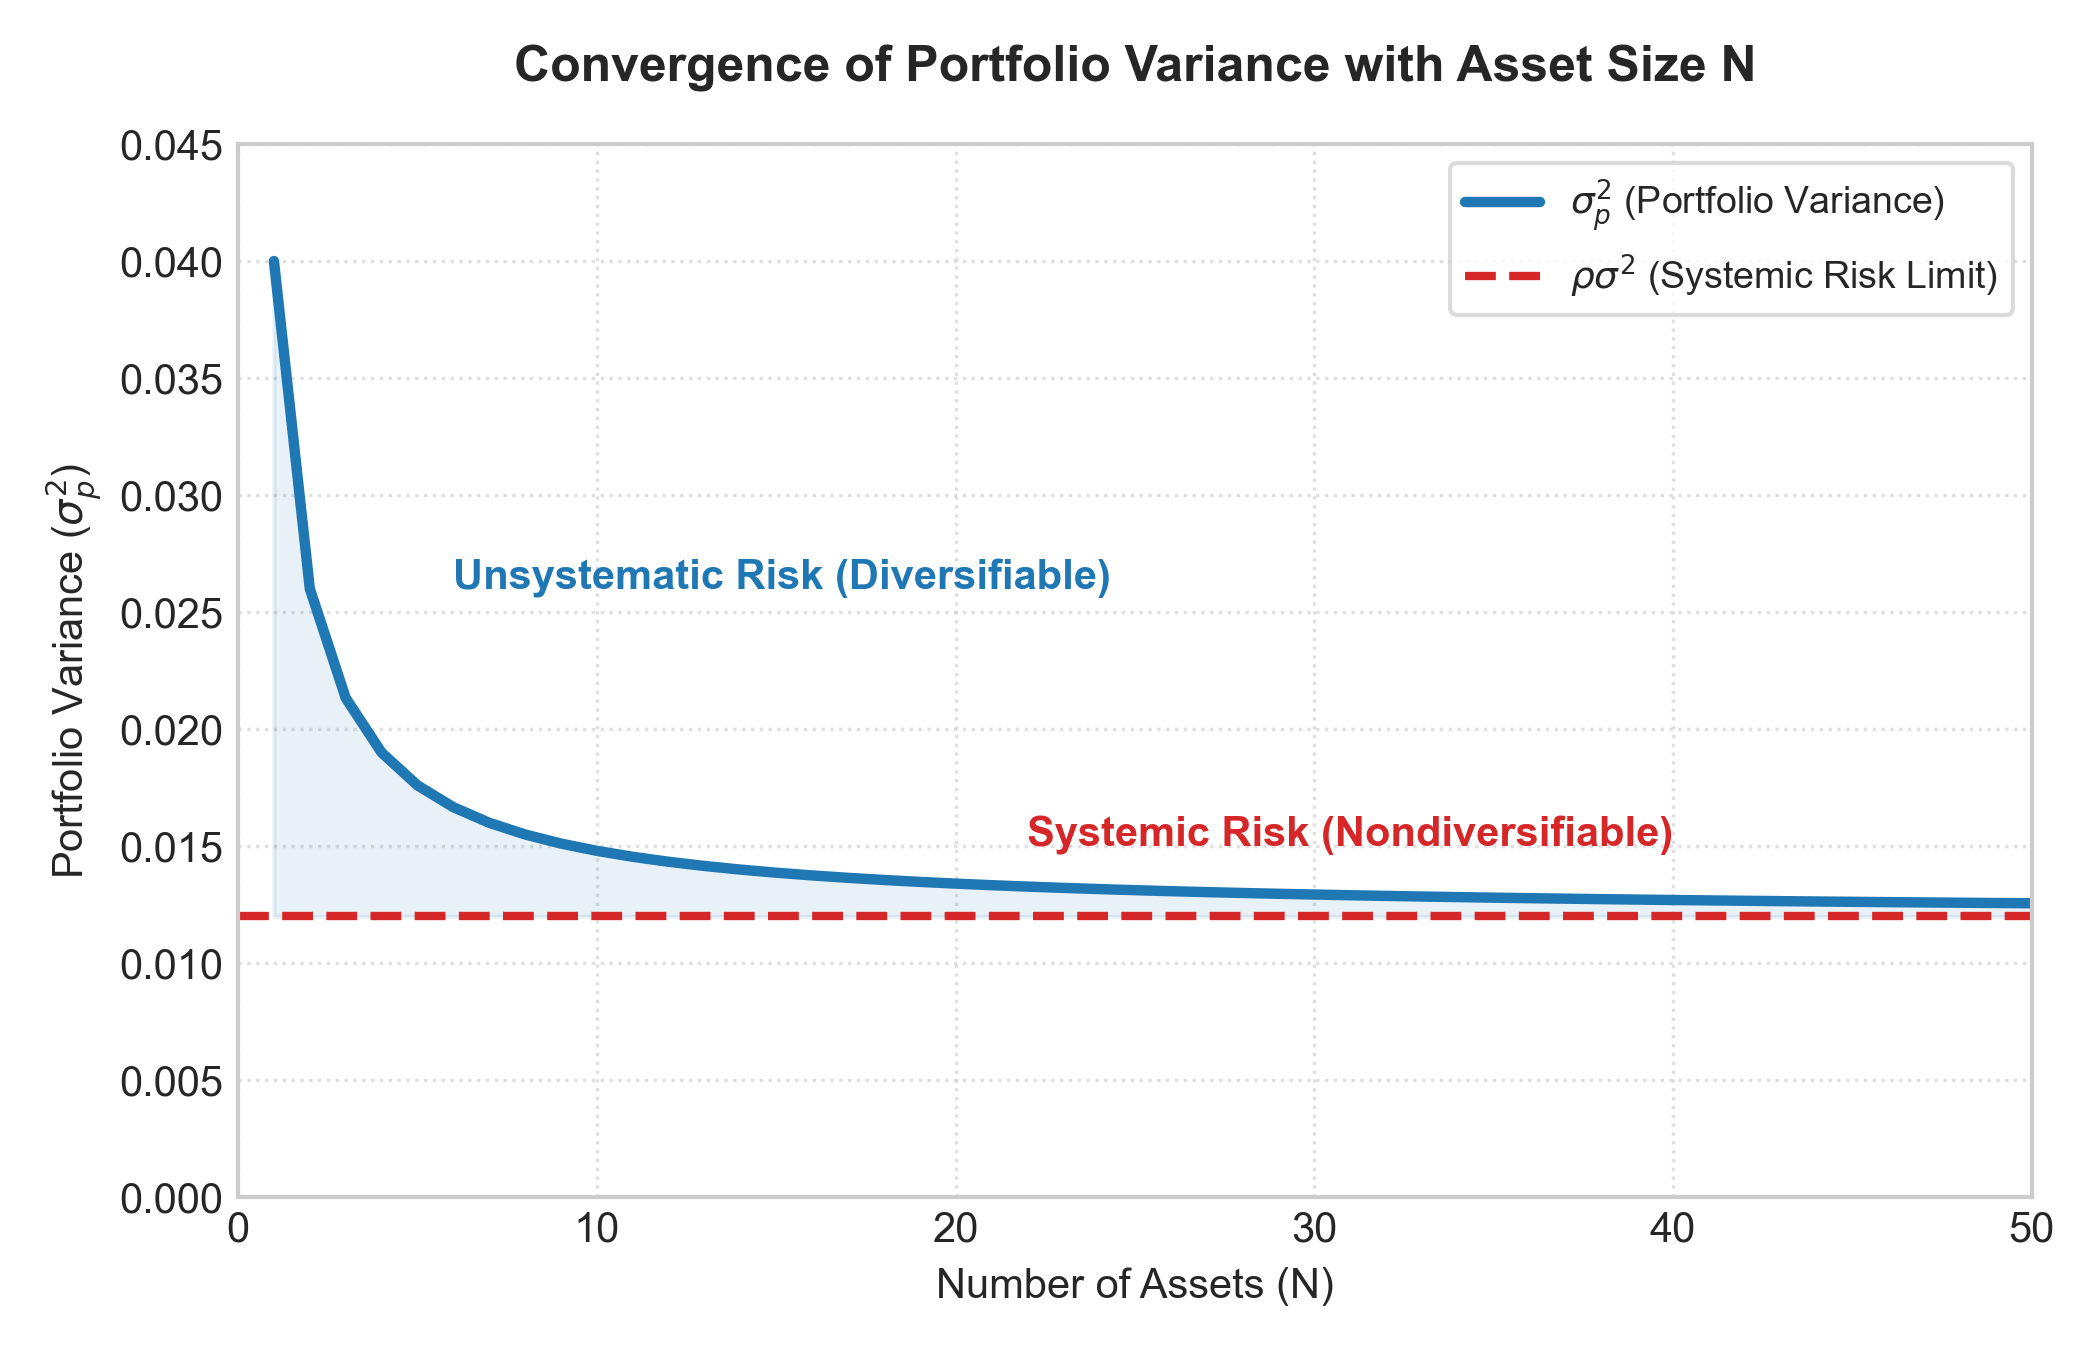
\includegraphics[width=0.65\textwidth]{figure/convergence.png}
\end{figure}

图1: 投资组合方差随资产数量N 的收敛轨迹

\begin{table}[ht]
  \centering
  \caption{表17: 等权组合方差收敛历程}
  \renewcommand{\arraystretch}{1.4}
\begin{tabularx}{\textwidth}{lYY}
  \toprule
  资产数量N & 组合方差$\sigma_p^2$大小 & 风险被分散化的物理状态 \\
  \midrule
  1 & $\sigma^2$ & 未进行配置,承担单资产全部波动风险。 \\
  2 & $\rho\sigma^2 + \dfrac{1}{2}(1 - \rho)\sigma^2$ & 第一期非系统性风险被消除一半。 \\
  10 & $\rho\sigma^2 + \dfrac{1}{10}(1 - \rho)\sigma^2$ & 随着N增加,非系统性风险大部分被消减。 \\
  N$\rightarrow$∞ & $\rho\sigma^2$(系统性风险下限) & 非系统性风险完全为0,收敛至系统性风险下限。 \\
  \bottomrule
\end{tabularx}
\end{table}

\section{资产组合风险二分法：系统性与非系统性风险}

\begin{table}[ht]
  \centering
  \caption{表18: 系统性风险与非系统性风险比对分析}
  \renewcommand{\arraystretch}{1.4}
\begin{tabularx}{\textwidth}{llYYY}
  \toprule
  风险类别 & 别称/标签 & 产生根源及物理背景 & 是否能分散消除 & 现实典型例证 \\
  \midrule
  系统性风险 & 市场风险/不可分散风险 & 全局性、宏观性因子变化,同时波及所有资产。 & 否 & 央行利率变动、通胀、汇率危机、地缘政治冲突。 \\
  非系统性风险 & 特质性风险/公司特有风险 & 单一公司所独有的微观突发事件。 & 是 & 核心技术研发失败、高管流失、财务造假曝光。 \\
  \bottomrule
\end{tabularx}
\end{table}

\section{现代资产组合理论假设前提与效用函数}

\subsection{MPT 核心假设前提}

1. 理性与风险厌恶：投资者皆为风险厌恶型，偏好高收益、惧怕高风险。 

2. 正态分布假定：资产回报均服从正态分布，因而仅需使用期望值与方差描述。 

3. 均值-方差决策准则：在收益相同下选择风险最小组合，在风险相同下选择收益最大组合。 

\subsection{投资者的效用函数模型}

对于风险厌恶的理性投资者，其效用在承受收益方差 $\sigma _ { p } ^ { 2 }$ 的惩罚下（风险厌恶系数 $A$ > 0） 定义为： 

\textbf{\color{UnivColor} 【均值-方差效用函数模型】} 

$$
\boxed {U = E (r _ {p}) - \frac {1}{2} A \sigma_ {p} ^ {2}}
$$

$$
\boxed {E (r _ {p}) = U + \frac {1}{2} A \sigma_ {p} ^ {2}}
$$

\begin{figure}[ht]
  \centering
  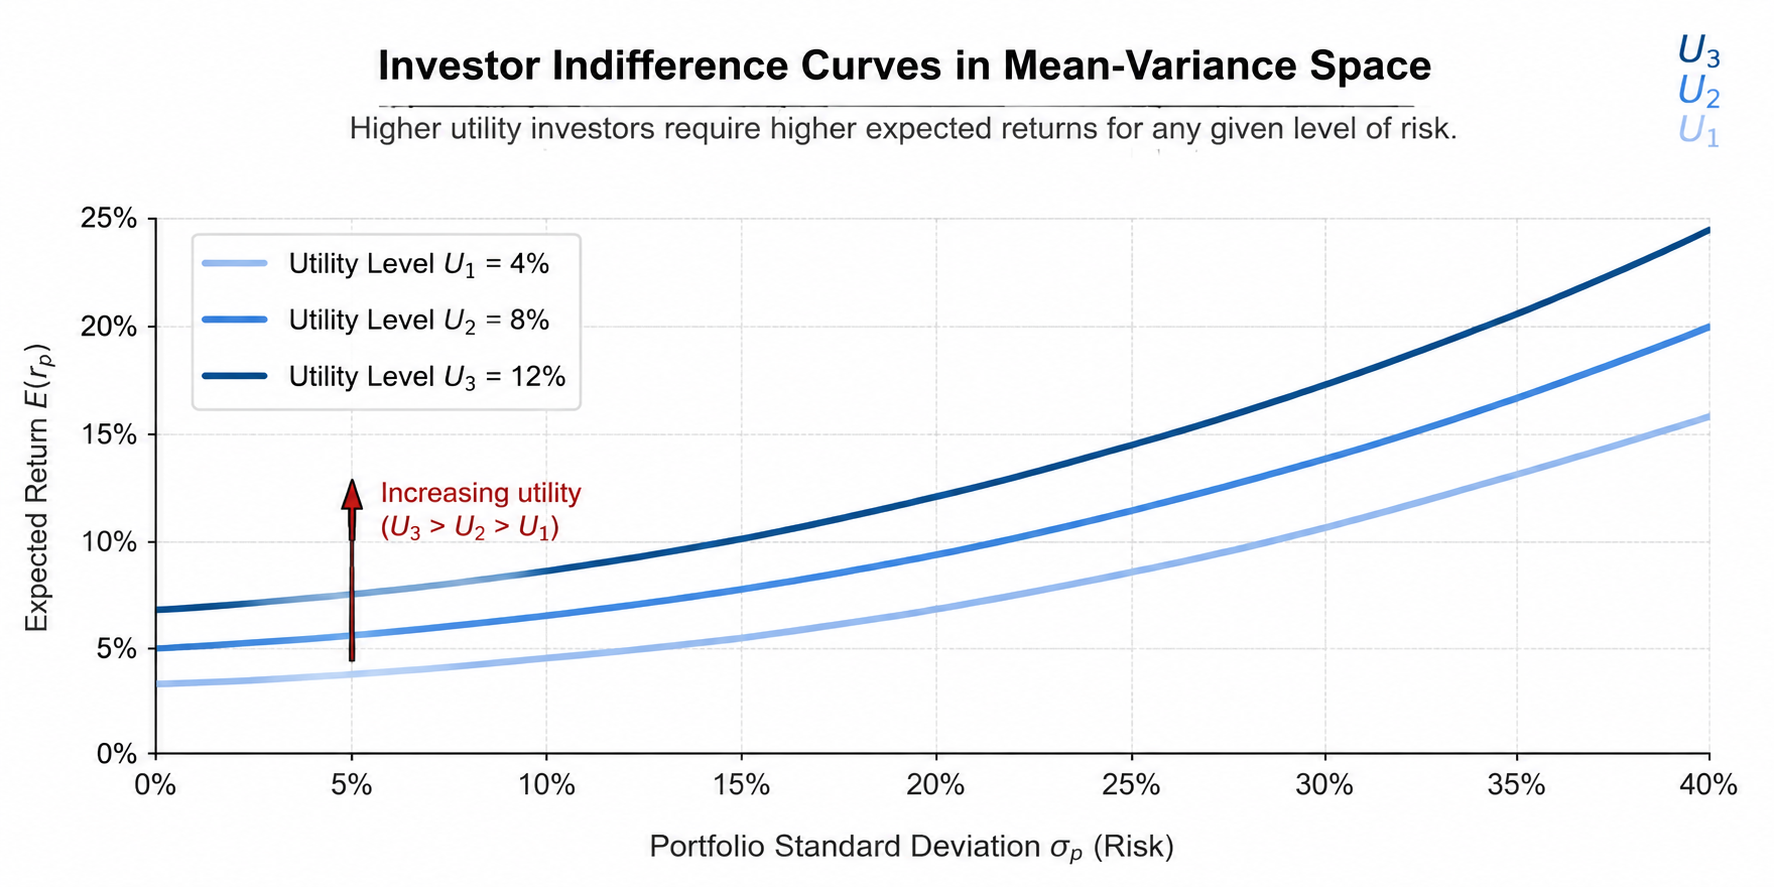
\includegraphics[width=0.65\textwidth]{figure/indifference.png}
\end{figure}

图2: 风险厌恶投资者的均值-方差无差异曲线分布

\section{风险资产与无风险资产的资产配置（CAL）}

\subsection{无风险资产属性与组合特征}

无风险资产拥有确定性收益 $r _ { f }$ 并且波动方差为 0： $E ( r _ { f } ) = r _ { f } , \sigma _ { f } ^ { 2 } = 0$ 。当把自有资金按 w 比例投向风险组合，其余 $1 - w$ 投向无风险资产时，资产配置性质如下： 

\textbf{\color{UnivColor} 【资本配置线、夏普比率与最优配置权重模型】} 

$$
E (r _ {p}) = r _ {f} + \left[ \frac {E (r _ {s}) - r _ {f}}{\sigma_ {s}} \right] \sigma_ {p}
$$

$$
\text { Sharpe   Ratio } = \frac {E (r _ {s}) - r _ {f}}{\sigma_ {s}}
$$

$$
w ^ {*} = \frac {E (r _ {s}) - r _ {f}}{A \sigma_ {s} ^ {2}}
$$

\begin{table}[ht]
  \centering
  \caption{表 19: 配置权重区间与经济含义}
  \renewcommand{\arraystretch}{1.4}
\begin{tabularx}{\textwidth}{lYY}
  \toprule
  配置权重w物理大小 & 现实金融交易含义 & 投资组合杠杆状态 \\
  \midrule
  w=0 & 100\%资金均买入国债等无风险资产。 & 无杠杆,无风险。 \\
  $0 < w < 1$ & 资金分仓买入风险资产与国债。 & 无杠杆防御型分仓配置。 \\
  w=1 & 满仓买入风险资产。 & 无负债杠杆。 \\
  w>1 & 借入资金(卖空无风险资产)投资风险资产。 & 融资杠杆交易 \\
  \bottomrule
\end{tabularx}
\end{table}

\section{资产配置的理论与现实意义}

现代资产组合理论为后续金融学科分支的发展奠定了关键基础，衍生出两条核心研究路径： 

1. 主动风险管理：资产配置通过跨市场、多元对冲、期货与期权等衍生工具消减非系统性风 险，并在剩余风险预算下最大化夏普比率。 

2. 资产资本定价：由于非系统性风险可以通过免费的分散化被完美消除，资本市场只愿意为 投资者承担的系统性风险支付对价（超额溢价）。这一革命性思想直接启发了后续的资本 资产定价模型 (CAPM)与套利定价理论 (APT)。 

\section{经典真题解析与思路串讲}

案例 14 (2019 清华：多期几何收益年化计算). 某投资者在第 1 年初以每股 80 美元购入 100 股 A公司股票，A公司在持有期内不分红。已知年末股价变动路径依次为100美元、120美元、150 美元，在第 4 年末股价回落至 100 美元并悉数卖出。求该投资在这 4 年期间的几何年化平均收 益率为多少？（） 

A. 0.0\% 

B. 1.0\% 

C. 5.7\% 

D. 9.2\% 

\textbf{\color{UnivColor} 【答案】} C 

\textbf{\color{UnivColor} 【解析】}几何收益率仅与买入价 $P _ { 0 }$ 和期末卖出价 $P _ { 4 }$ 相关，与持有期间的中间股价波动路径无 关： 

$$
\begin{aligned}
  (1 + \bar {r} _ {G}) ^ {4} &= \frac {P _ {4}}{P _ {0}} = \frac {1 0 0}{8 0} = 1. 2 5 \\[1.2ex]
  &\Rightarrow \quad \boxed {\bar {r} _ {G} = \left(\frac {100}{80}\right) ^ {1 / 4} - 1 \approx 5.74 \%}
\end{aligned}
$$

故选 C。 

案例15(2022 上财：完全负相关组合对冲测算). 在两资产组合中，资产A的标准差为 $\sigma _ { A } = 6 0 \%$ ， 资产 B 的标准差为 $\sigma _ { B } = 4 0 \%$ 。两资产完全负相关。若在组合中 A 权重为 $w _ { A } = 2 5 \%$ , B 权重为 $w _ { B } = 7 5 \%$ 。求此配置组合的标准差。 

A. 10.0\% 

B. 15.0\% 

C. 20.0\% 

D. 25.0\% 

\textbf{\color{UnivColor} 【答案】} B 

\textbf{\color{UnivColor} 【解析】} 完全负相关（相关系数ρ = -1）下，组合标准差适用完全对冲化简公式： 

$$
\sigma_ {p} = | w _ {A} \sigma_ {A} - w _ {B} \sigma_ {B} | = | 25 \% \times 60 \% - 75 \% \times 40 \% | = | 15 \% - 30 \% | = 15 \%
$$

案例 16 (2019 上财：完全负相关与目标收益解权重). 已知股票 A 预期回报 $E ( r _ { A } ) = 1 2 \%$ ，标 准差 $\sigma _ { A } = 1 5 \%$ ；股票 B 预期回报 $E ( r _ { B } ) = 2 0 \%$ ，标准差 $\sigma _ { B } = 4 5 \%$ 。两股票完全负相关。现欲 构建一个预期年化收益率为16\% 的组合，求该投资组合的方差为多少？ 

A. 0.0225 

B. 0.0324 

C. 0.0357 

D. 0.0431 

\textbf{\color{UnivColor} 【答案】} A 

\textbf{\color{UnivColor} 【解析】} 

1. 利用期望收益率公式解出资产配置权重 $w _ { A }$ ： 

$$
\begin{aligned}
  16 \% &= 12 \% w _ {A} + 20 \% (1 - w _ {A}) \\[1.2ex]
  &\Rightarrow \quad 1 6 = 2 0 - 8 w _ {A} \\[1.2ex]
  &\Rightarrow \quad \boxed {w _ {A} = 50 \%}
\end{aligned}
$$

即股票 B 的权重 $w _ { B } = 1 - w _ { A } = 5 0 \%$ 。 

2. 代入相关系数 $\rho$ = -1 下的标准差对冲公式： 

$$
\sigma_ {p} = | w _ {A} \sigma_ {A} - w _ {B} \sigma_ {B} | = | 50\% \times 15\% - 50\% \times 45\% | = | 7.5\% - 22.5\% | = 15\%
$$

3. 计算组合方差： 

$$
\sigma_ {p} ^ {2} = (15\%) ^ {2} = 0. 0 2 2 5
$$

案例 17 (2019 清华：马科维茨协方差矩阵项数计数). 在马科维茨组合理论中，包含 N 种资产 的方差-协方差矩阵共有 $N ^ { 2 }$ 个元素。则矩阵中不重复的、位于非对角线上的协方差项数共有多 少项？ 

A. $N^2$ 

B. N 

C. $N ^ { 2 } - N$ 

D. $\frac{N^2 - N}{2}$ 

\textbf{\color{UnivColor} 【答案】} C 

\textbf{\color{UnivColor} 【解析】}方差-协方差矩阵的对角线上是N 个资产各自的方差项。其余非对角线上的 $N ^ { 2 } - N$ 个 元素代表资产两两之间的协方差项。由于矩阵对称性（$\operatorname{Cov}(r_i, r_j) = \operatorname{Cov}(r_j, r_i)$），共有 $N^2 - N$ 项（若问不重复的独立协方差项，则是 $\frac{N^2 - N}{2}$ ，本题对应题意非对角线元素项数，故为 $N^2 - N$）。

\end{document}
